\documentclass{beamer}

\usepackage{subcaption}
\usepackage{graphicx}
\usepackage{pgfgantt}
\graphicspath{{src/}}

\usepackage[bottom]{footmisc}
\usetheme{Boadilla}

\AtBeginSection[]
{
  \begin{frame}
    \frametitle{Table of Contents}
    \tableofcontents[currentsection]
  \end{frame}
}

\title{PhD proposal}
\subtitle{for research in wireless information and power transfer}

\author{Yang Zhao}
\date{15 Aug 19}

\begin{document}

\frame{\titlepage}



\section{Background}
\subsection{Education experience}

\begin{frame}
\frametitle{Education and work experience}

%% Education
\begin{block}{Education}

\begin{minipage}[t]{0.7\textwidth}
\flushleft{\textbf{Imperial College London}}
\end{minipage}
~
\begin{minipage}[t]{0.2\textwidth}
\flushright{2018 -- 2019}
\end{minipage}

\textit{MSc Communications and Signal Processing, expected distinction} \\

\begin{minipage}[t]{0.7\textwidth}
\flushleft{\textbf{University of Liverpool}}
\end{minipage}
~
\begin{minipage}[t]{0.2\textwidth}
\flushright{2016 -- 2018}
\end{minipage}

\textit{BEng Communications and Electronics, with distinction} \\

\begin{minipage}[t]{0.7\textwidth}
\flushleft{\textbf{Xi'an Jiaotong-Liverpool University}\footnotemark}
\end{minipage}
~
\begin{minipage}[t]{0.2\textwidth}
\flushright{2014 -- 2016}
\end{minipage}

\textit{BEng Telecommunications, with distinction}
\footnotetext{\tiny A UK-China 2+2 bachelor programme}
\end{block}

\end{frame}


\begin{frame}
\frametitle{Work experience}

%% Work
\begin{block}{Internship}

\begin{minipage}[t]{0.7\textwidth}
\flushleft{\textbf{China Mobile Group}}
\end{minipage}
~
\begin{minipage}[t]{0.2\textwidth}
\flushright{Jun 2018}
\end{minipage}

\textit{  - Network maintainer}

\begin{itemize}
  \item Deployed emergency response vehicles for events
  \item Maintained base stations
  \item Investigated the coverage of smartcells
\end{itemize}



\begin{minipage}[t]{0.7\textwidth}
\flushleft{\textbf{China Mobile Group Design Institute}}
\end{minipage}
~
\begin{minipage}[t]{0.2\textwidth}
\flushright{Jul 2017}
\end{minipage}

\textit{  - Assistant}

\begin{itemize}
  \item Summarized business solutions of NB-IoT and FDD LTE
  \item Simulated FDD coverage of Guangdong Province with tower and cell distribution
  \item Measured LTE performance (RSRP, SINR, CSFB rates) for F and D bands in typical regions
\end{itemize}

\end{block}

\end{frame}



\subsection{Courses}

\begin{frame}
\frametitle{Courses}

%% Courses
\begin{itemize}
  \item \alert{Antennas and array processing}
  \item Communication systems
  \item Computer vision
  \item Data structure and microprocessors
  \item Electromagnetics and RF engineering
  \item \alert{Information and coding theory}
  \item Instrumentation and control
  \item Integrated circuits
  \item Machine learning
  \item Power systems
  \item Probability and stochastic processes
  \item Signal processing
  \item \alert{Wireless communications}
\end{itemize}

\end{frame}


\subsection{Skills and honors}

\begin{frame}
\frametitle{Skills and honors}

%% Skills
\begin{block}{Skills (in descending order)}
\begin{itemize}
  \item Data collection and analysis
  \item Comprehension and innovation
  \item Asking questions
  \item Programming
  \item Self-learning
  \item Academic writing
  \item Communication and collaboration
  \item Project management
  \item Critical thinking
\end{itemize}
\end{block}

%% Honors
\begin{block}{Honors}
\begin{minipage}[t]{0.7\textwidth}
\flushleft{\textit{University achievement award}}
\end{minipage}
~
\begin{minipage}[t]{0.2\textwidth}
\flushright{2016}
\end{minipage}


\begin{minipage}[t]{0.7\textwidth}
\flushleft{\textit{IET student prize}}
\end{minipage}
~
\begin{minipage}[t]{0.2\textwidth}
\flushright{2018}
\end{minipage}

\end{block}

\end{frame}



\section{Research experience}

\subsection{Cross-Layer Optimization for 4G Broadband Wireless Communication Networks}

\begin{frame}
\frametitle{Cross-Layer Optimization for 4G Broadband Wireless Communication Networks}

\begin{block}{Why?}
\begin{itemize}
  \item To meet requirements of various services
  \item To improve system performance (throughput, delay, packet drop rate)
  \item To increase spectrum and power efficiency
\end{itemize}
\end{block}

\begin{block}{Where?}
\begin{itemize}
  \item Downlink traffic in OFDM systems
  \item PHY layer (CSI, capacity)
  \item MAC layer (traffic characteristics)
\end{itemize}
\end{block}

\begin{block}{What?}
\begin{itemize}
  \item Joint optimization of resource allocation and data scheduling
  \item Adaptive algorithms with low complexity
  \item Adjustable weight configuration (queue- and packet-based)
\end{itemize}
\end{block}

\end{frame}


\begin{frame}
\frametitle{Algorithms}

\begin{block}{Subcarrier allocation}
\begin{itemize}
  \item Maximum Weighted Capacity (MWC): balance QoS and capacity
  \item Proportional Fairness (PF): equalize rate for users
\end{itemize}
\end{block}

\begin{block}{Power allocation}
\begin{itemize}
  \item Weighted Water-Filling (WWF): based on subcarrier allocation under equal power assumption (low-complexity but suboptimal)
\end{itemize}
\end{block}

\begin{block}{Data scheduling}
\begin{itemize}
  \item Modified Largest Weighted Delay First (M-LWDF): serve the queues on service nature, delay, and queue length
  \item Packet Dependent (PD): data is sent packet by packet with individual weight design (depends on QoS, delay, and packet size)
\end{itemize}
\end{block}

\end{frame}


\begin{frame}
\frametitle{Conclusion and limitations}

We investigated the performance for conventional services (background, voice, video) and extended the research to networks with haptic traffic.

\begin{block}{Conclusion}
\begin{itemize}
  \item With a flexible transmission scheme, PD provides larger throughput and lower packet drop rate than M-LWDF, especially for heavy traffic (large number of users, low SNR, multiple service types).
  \item By properly choosing the number of packets for weight calculation, the proposed design requires lower overall complexity than conventional queue-based ones.
  \item The low-complexity suboptimal power allocation performs similarly to the optimal strategy, as subcarrier allocation has more significant impact on system performance.
\end{itemize}
\end{block}

\begin{block}{Limitations}
\begin{itemize}
  \item Only SISO case is considered.
  \item There exists fairness issues.
\end{itemize}
\end{block}

\end{frame}



\subsection{Signal Optimization for Wireless Information and Power Transmission}

\begin{frame}
\frametitle{Signal Optimization for Wireless Information and Power Transmission}

\begin{block}{Why?}
\begin{itemize}
  \item To provide perpetual and reliable energy supply for low-power devices
  \item To reduce the use of batteries and get rid of wires, with increased operation range
  \item To improve rate-energy tradeoff in WIPT
\end{itemize}
\end{block}

\begin{block}{Where?}
\begin{itemize}
  \item Transmitter (waveform design, resource allocation)
  \item Receiver (information decoding (ID) and energy harvesting (EH))
\end{itemize}
\end{block}

\begin{block}{What?}
\begin{itemize}
  \item Nonlinear harvester model and superposed waveform
  \item Fundamental dependency of harvested power on signal design
  \item Waveform optimization and rate-energy region characterization
\end{itemize}
\end{block}

\end{frame}


\begin{frame}
\frametitle{System architecture}

\begin{figure}
  \centering
    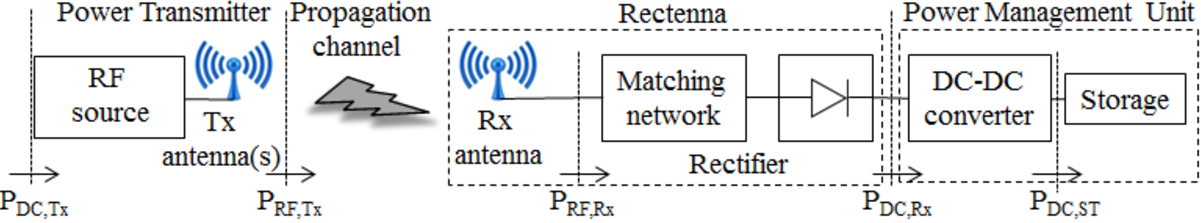
\includegraphics[width=\textwidth]{wpt_block_diagram}
  \caption{Block diagram of WPT \cite{Clerckx2018a}}
  \label{fig:wpt-block-diagram}
\end{figure}

\textbf{RF-to-DC conversion efficiency ${e_3}$}: \alert{rectenna} and \alert{waveform design}

\end{frame}


\begin{frame}
\frametitle{Rectenna model}

\begin{figure}
  \centering
    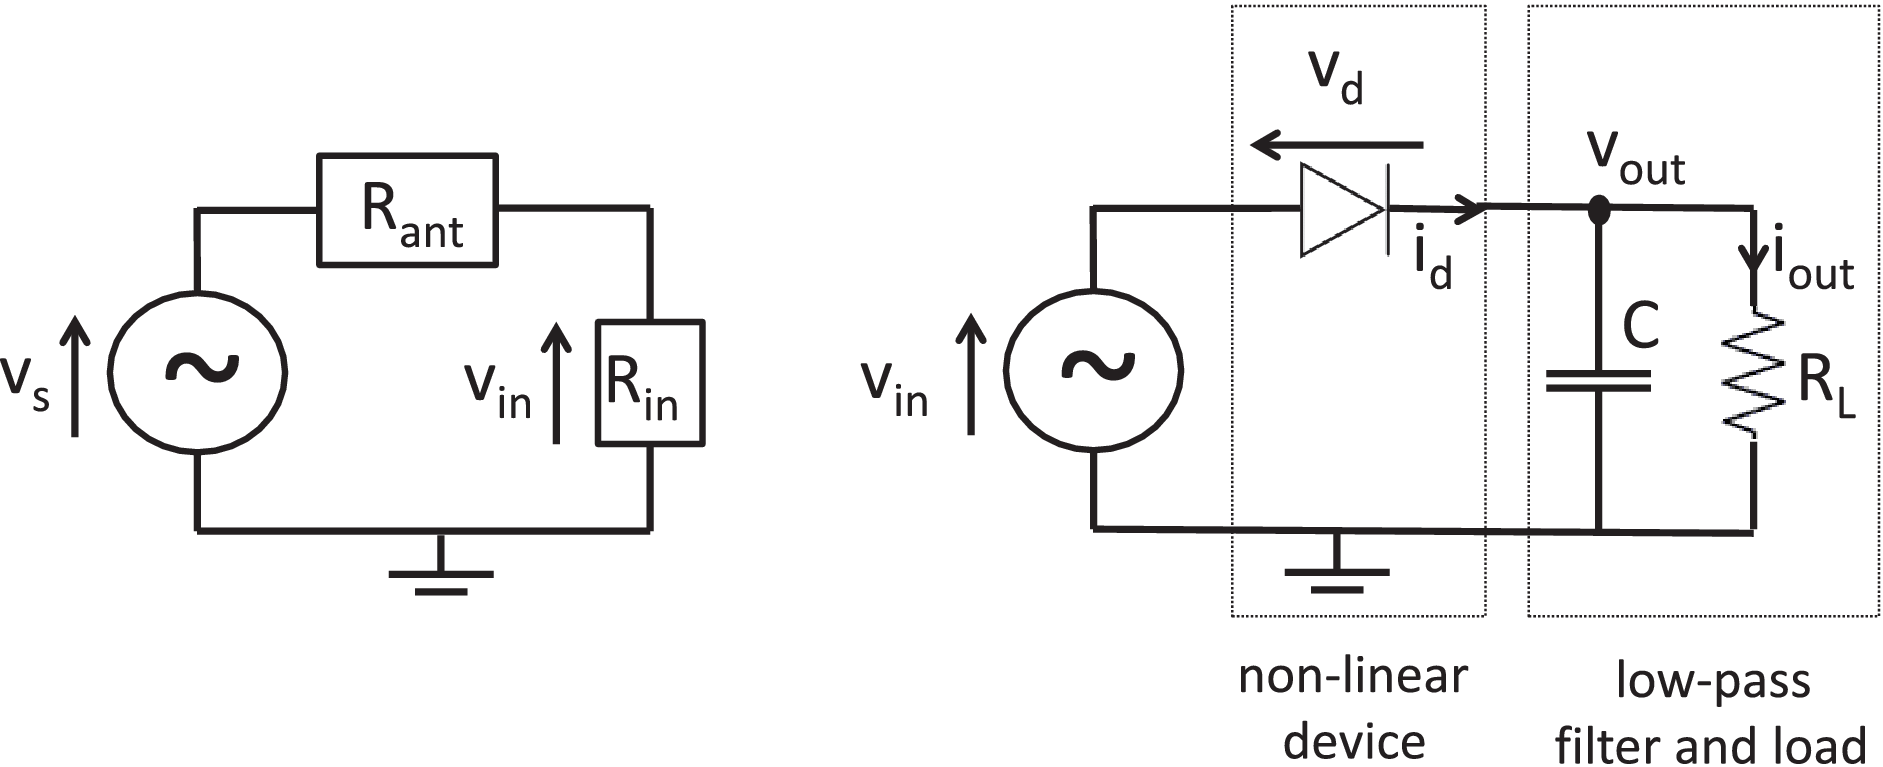
\includegraphics[width=0.8\textwidth]{rectenna_circuit}
  \caption{Rectenna equivalent circuit (left) and a single diode rectifier (right) \cite{Clerckx2018a}}
  \label{fig:rectenna_circuit}
\end{figure}

\begin{itemize}
  \item Diodes account for the nonlinearity
  \item Taylor expansion of diode characteristic equation (small-signal model)
  \item Truncate to the ${n_o}$-th order
  \begin{itemize}
    \item diode linear model (${n_o} = 2$): output power is proportional to input power
    \item diode nonlinear model (${n_o} > 2$): significant contributions of higher order terms
  \end{itemize}
\end{itemize}

\end{frame}


\begin{frame}
\frametitle{Waveform design and receiver architecture}

A superposed signal containing \alert{modulated information waveform} and \alert{multisine power waveform} is demonstrated to bring a two-fold benefit:

\begin{block}{Benefits of proposed waveform}
\begin{itemize}
  \item \textbf{rate}: multisine is deterministic with no interference on information component
  \item \textbf{energy}: multisine reduce the threshold to enjoy the benefit of diode nonlinear model (-20 dBm to -30 dBm)
\end{itemize}
\end{block}

Two receiver architectures are available:

\begin{block}{Receiver architectures}
\begin{itemize}
  \item Time Switching (TS): switch between EH and ID on time basis
  \item Power Splitting (PS): split the received signal into separate portions
\end{itemize}
\end{block}

\end{frame}


\begin{frame}
\frametitle{Multisine}

\begin{figure}
  \centering

  \begin{subfigure}{.35\textwidth}
    \centering
      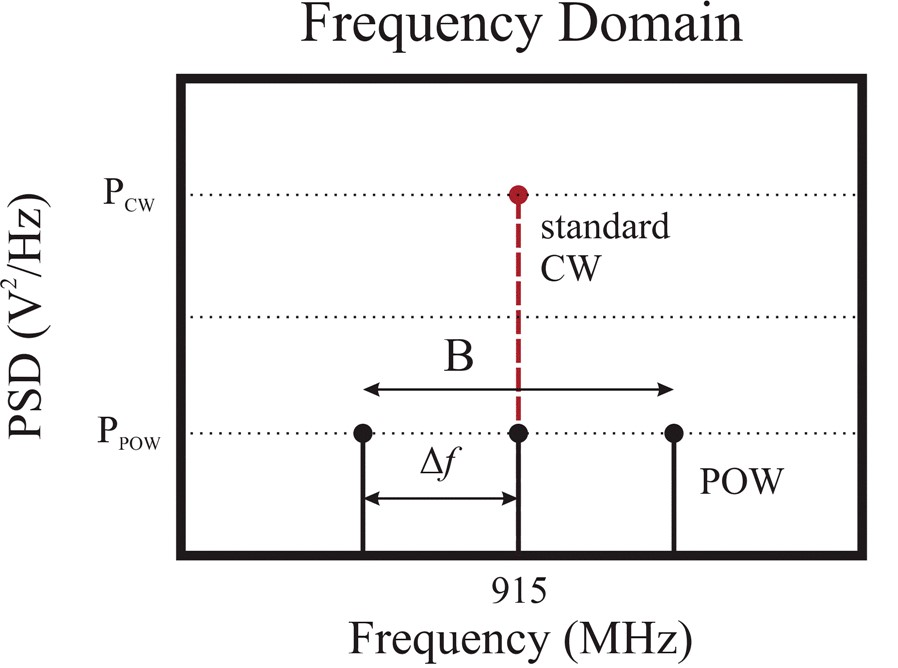
\includegraphics[width=\textwidth]{waveform_frequency_domain}
    \caption{Frequency domain}
    \label{fig:waveform_frequency_domain}
  \end{subfigure}
  \begin{subfigure}{.35\textwidth}
    \centering
      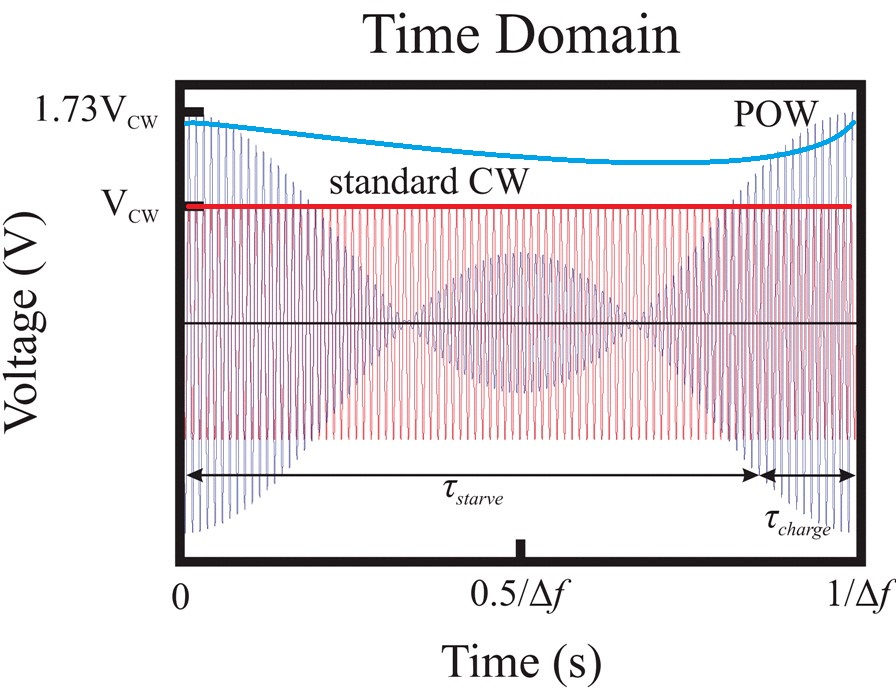
\includegraphics[width=\textwidth]{waveform_time_domain}
    \caption{Time domain}
    \label{fig:waveform_time_domain}
  \end{subfigure}

  \caption{Comparison of 3-subcarrier multisine and continuous wave (modified from \cite{Trotter2009}). The thick lines are typical rectifier output voltage.}
  \label{fig:waveform_comparison}
\end{figure}

\begin{block}{Characteristics}
\begin{itemize}
  \item High peak-to-average power ratio (PAPR)
  \item Concentrated power triggers the diode
  \item Pulse amplitude determined by number of tones $N$
\end{itemize}
\end{block}

\end{frame}


\begin{frame}
\frametitle{Algorithms}

The optimization is based on geometric programming (GP) using CVX. We aim to maximize harvested current subject to transmit power and rate constraints. The following cases are being investigated:

\begin{block}{Algorithms}
\begin{itemize}
  \item Decoupling spatial and frequency design
  \item Lower-bound (assume interference from power waveform)
  \item No multisine waveform
  \item PAPR constraint
  \item MIMO (suboptimal by GP)
\end{itemize}
\end{block}

\end{frame}


\begin{frame}
\frametitle{Conclusion and limitations}

We explored the impact of subcarrier number and SNR on rate-energy tradeoff. PAPR and MIMO require further simulations.

\begin{block}{Conclusion}
\begin{itemize}
  \item With a large number of subcarrier ($N \geqslant 4$), the superposed waveform is useful to enlarge the rate-energy region.
  \item TS is favoured for large $N$ and low SNR; PS on the contrary.
  \item Number of Rx has significant influence on rate-energy tradeoff.
\end{itemize}
\end{block}

\begin{block}{Limitations}
\begin{itemize}
  \item GP is suboptimal for multiple Rx.
  \item The iterative algorithms are sensitive to initialization and take long time to solve for large $N$ and Rx.
  \item It requires perfect CSIT.
  \item (To be fixed) If initialized with previous solutions, the algorithm may collapse due to precision issues.
\end{itemize}
\end{block}

\end{frame}



\section{Proposal}
\subsection{Waveform and Transceiver Design for Dual Mode MIMO Wireless Information and Power Transfer}

\begin{frame}
\frametitle{Questions and ideas}

Let's start with some questions and novel ideas:

\begin{block}{Questions}
\begin{itemize}
  \item What's the optimal resource allocation strategy for MIMO?
  \item How to reduce the complexity while maintaining the performance?
  \item Are there any other harvester models?
\end{itemize}
\end{block}

\begin{block}{Ideas}
\begin{itemize}
  \item Improve RF-to-DC conversion efficiency with multiple rectifiers \cite{Ma2019}
  \item Encode information with PAPR of multisine rather than individual waveform \cite{Park2018, Krikidis2019}
  \item Switch between single and multi-tone transmission adaptively to CSI and rate requirement \cite{Park2018}
\end{itemize}
\end{block}

\end{frame}

\begin{frame}
\frametitle{Motivations}

\begin{block}{In industry}
\begin{itemize}
  \item To prolong the lifetime for mobile devices
  \item To reduce the cost in battery recharging and replacement
  \item To make devices smaller and lighter
\end{itemize}
\end{block}

\begin{block}{In academia}
\begin{itemize}
  \item To propose a low-complexity suboptimal waveform design for WIPT
  \item To investigate the performance of tone-index multisine modulation on FF and FS channels
  \item To explore the possibility of dual-mode WIPT for MIMO systems with multiple harvesters
\end{itemize}
\end{block}

\end{frame}


\begin{frame}
\frametitle{Proposed system architecture}

\begin{figure}
  \centering
    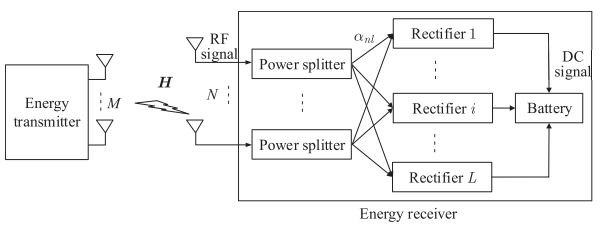
\includegraphics[width=0.8\textwidth]{system_architecture}
  \caption{System architecture of the MIMO multi-rectifier WIPT system \cite{Ma2019}}
  \label{fig:system_architecture}
\end{figure}

Each receive antenna is followed by a power splitter to reallocate the power:

\begin{itemize}
  \item when the received power level is relatively low, the splitters will combine all energy branches in one rectifier to enjoy the benefit of harvester nonlinearity.
  \item when the power is sufficiently high, the components will be equally divided to avoid the saturation of diode breakdown region.
\end{itemize}

\end{frame}


\begin{frame}
\frametitle{Transmitter}

\begin{figure}
  \centering
    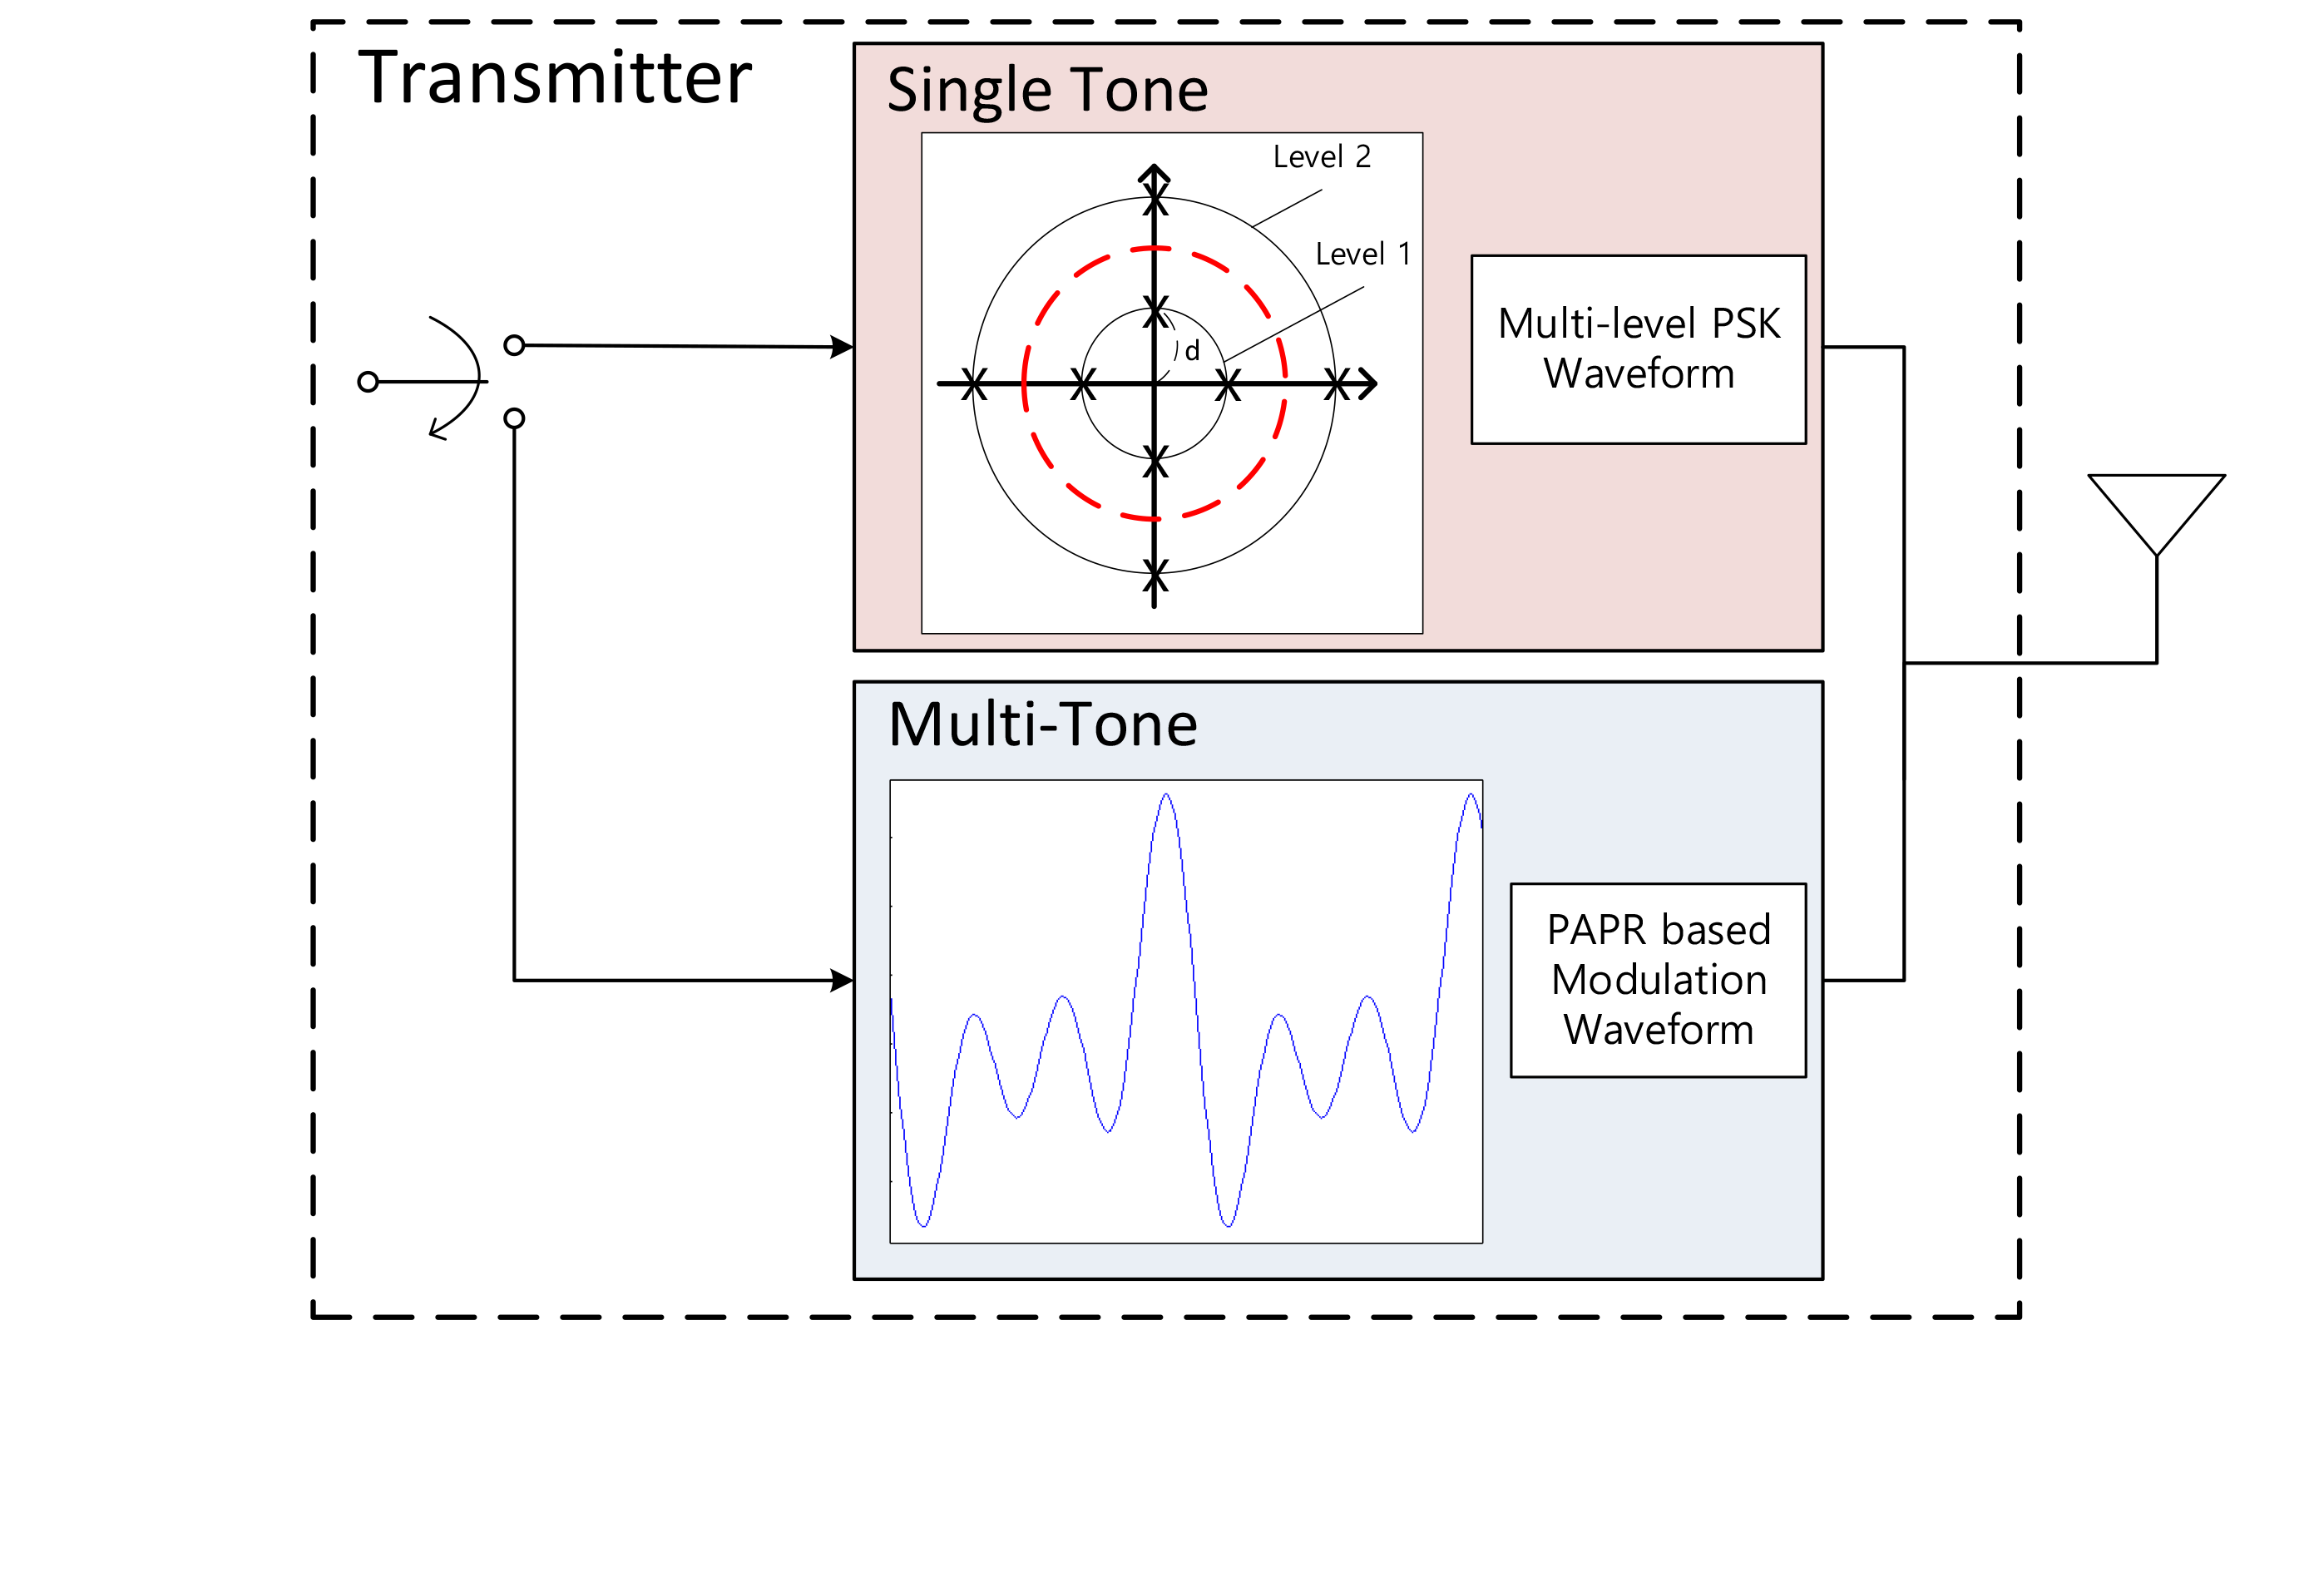
\includegraphics[width=0.8\textwidth]{transmitter}
  \caption{Transmitter architecture \cite{Park2018}}
  \label{fig:transmitter}
\end{figure}

\end{frame}


\begin{frame}

\begin{block}{Transmitted waveform}
\frametitle{Transmitter}

\begin{itemize}
  \item \textbf{single-tone}: phase- and amplitude-modulated, optimized for information transmission
  \item \textbf{multi-tone}: PAPR-modulated, optimized for power transmission
  \item The transmission mode depends on the adaptive mode-switching algorithm to design
\end{itemize}
\end{block}

\end{frame}


\begin{frame}
\frametitle{Receiver}

\begin{figure}
  \centering
    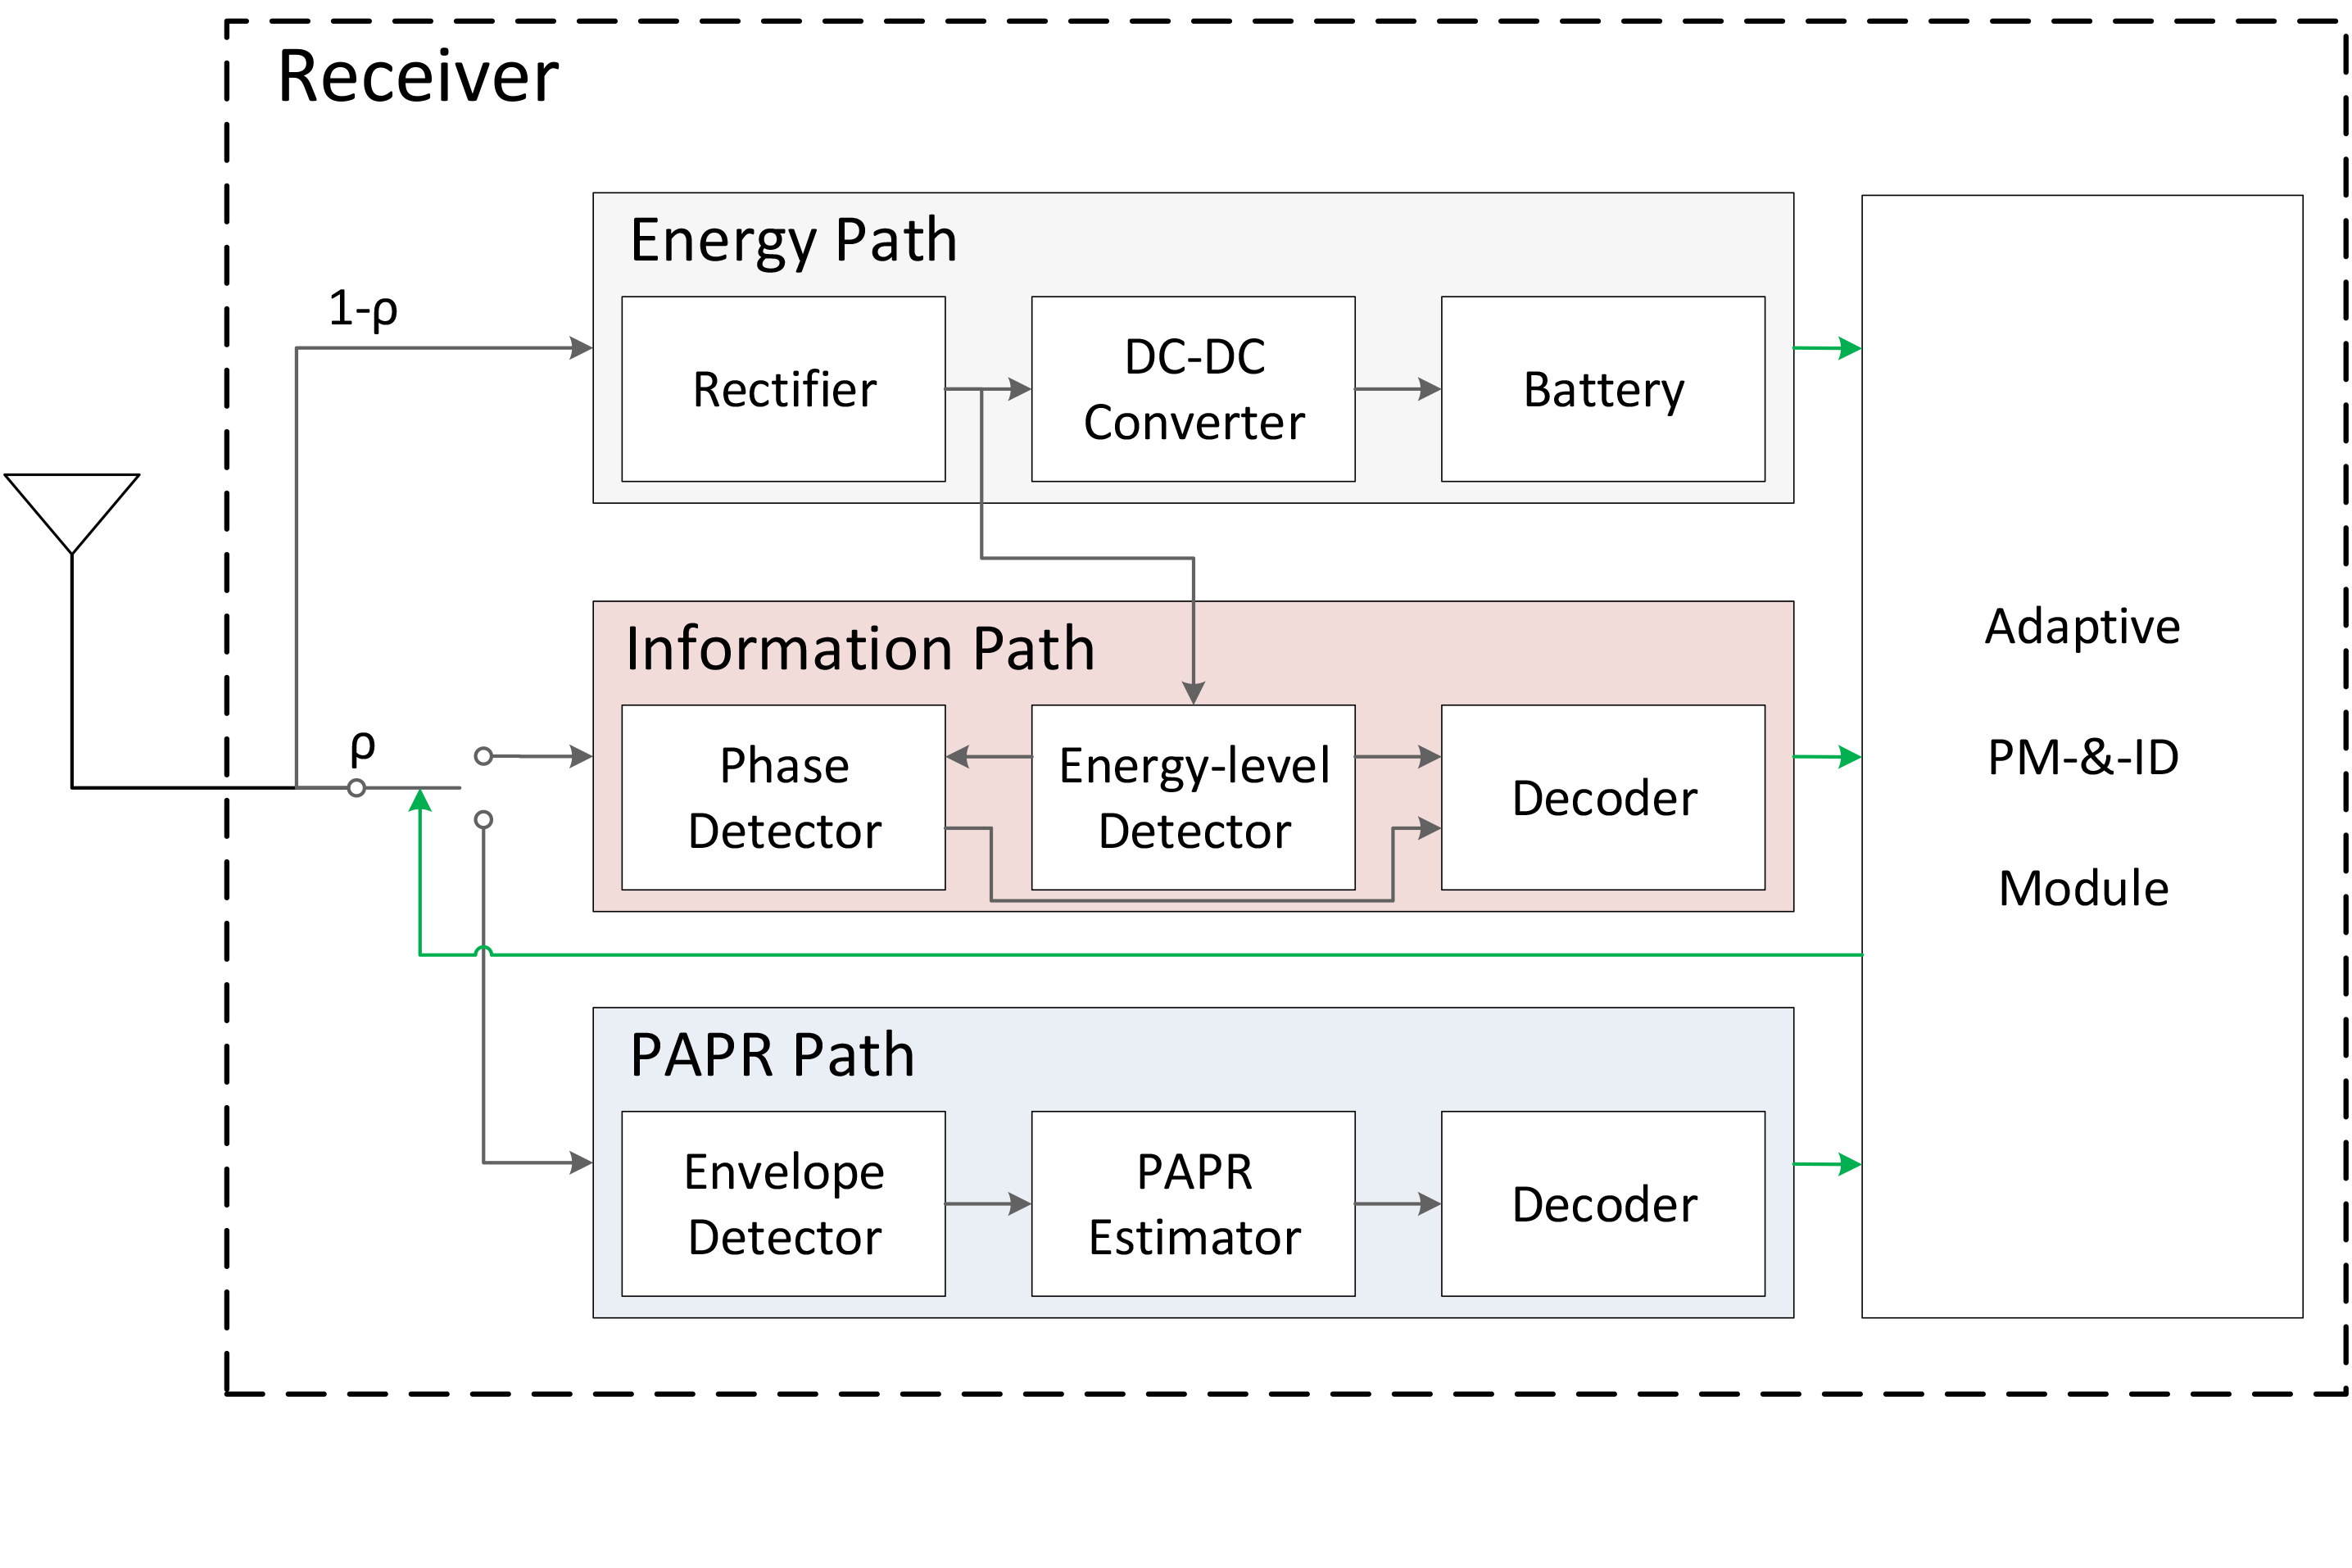
\includegraphics[width=0.8\textwidth]{receiver}
  \caption{Receiver architecture \cite{Park2018}}
  \label{fig:receiver}
\end{figure}

\end{frame}


\begin{frame}
\frametitle{Receiver}

\begin{block}{Receiver blocks}
\begin{itemize}
  \item \textbf{energy path}: harvest energy and supply information path or store in battery
  \item \textbf{information path}: demodulate phase and amplitude information [for single-tone mode]
  \item \textbf{PAPR path}: decode PAPR-based information [for multisine mode]
\end{itemize}
\end{block}

Two possible ways:

\begin{itemize}
  \item One unified energy path, harvests power only
  \item One energy path for each receiver, decodes amplitude information as well
\end{itemize}

\end{frame}


\begin{frame}
\frametitle{Comments}

\begin{block}{Advantages}
\begin{itemize}
  \item Optimization on the mode-switching design is with lower complexity than superposed waveform.
  \item We expect a significant larger rate-energy region with multi-harvester MIMO.
  \item The operation range can also be increased.
\end{itemize}
\end{block}

\begin{block}{Opportunities}
\begin{itemize}
  \item Harvester model: diode models vs logistic curve fitting models \cite{Boshkovska2015}
  \item CSIT: perfect vs imperfect
  \item Receiver strategy: PS, TS vs antenna switching \cite{Liu2013}
\end{itemize}
\end{block}

\end{frame}


\begin{frame}
\frametitle{Timeline}

\begin{figure}
  \centering
    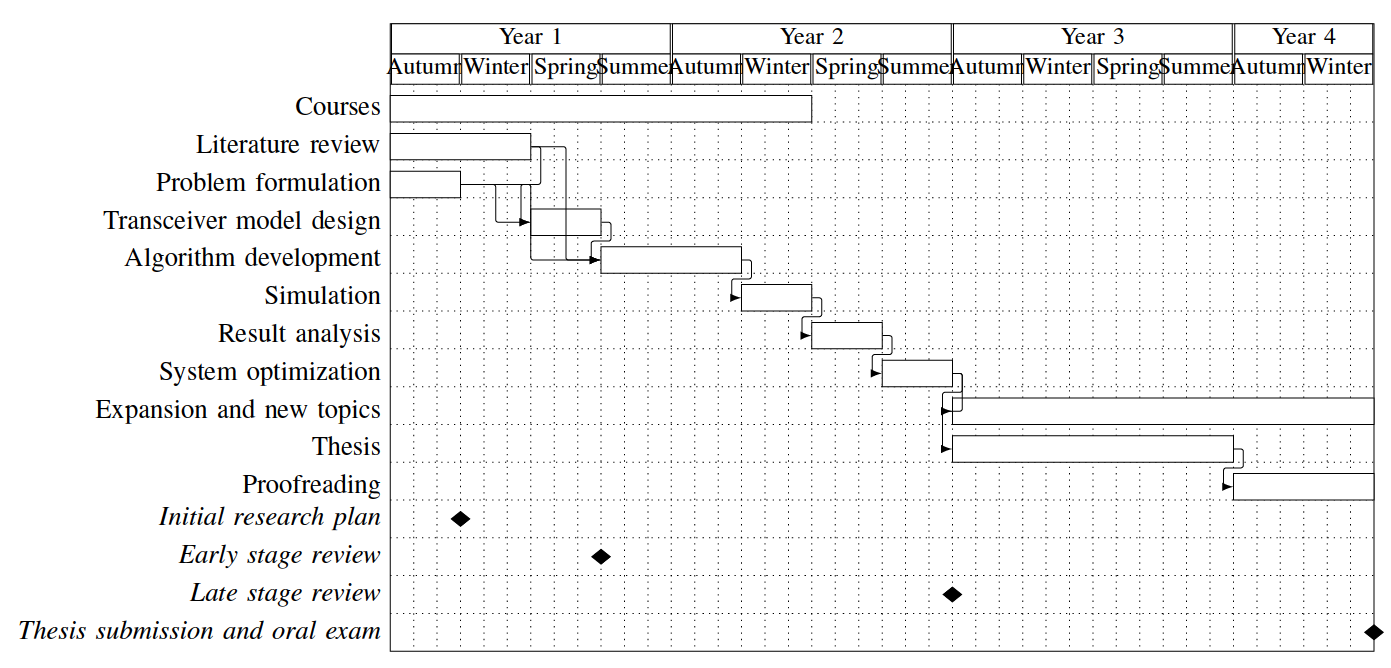
\includegraphics[width=\textwidth]{gantt_chart}
  \caption{Gantt chart of the project}
  \label{fig:gantt_chart}
\end{figure}

\end{frame}


\begin{frame}
  \centering
  \Large \emph{Thank you!}
\end{frame}

\bibliographystyle{IEEEtran}
\bibliography{library}

\end{document} 